\documentclass[t,xcolor={svgnames,table}]{beamer}

\mode<presentation>
\usetheme{Warsaw}
\usecolortheme[snowy]{owl}
\useoutertheme{infolines} 

\usepackage{lmodern}
\usepackage{amsmath}
\usepackage{amsfonts}
\usepackage{bbm}
\usepackage{bm}
\usepackage{nicefrac}
\usepackage{color}
\usepackage{multirow}
\usepackage{multicol}
\usepackage{adjustbox}
\usepackage{tikz}
\usepackage{tikz-dependency}
\usepackage{tikz-qtree}
\usepackage{pgfplots,pgfplotstable}
\usepackage{pgf}
\usepackage{collcell}
\usepackage{booktabs}
\usepackage{soul}
\usepackage{verbatim}

% colorblind friendly scheme generated by
% http://colorbrewer2.org/#type=qualitative&scheme=Dark2&n=3
\definecolor{yellow}{HTML}{d95f02}
\definecolor{green}{HTML}{1b9e77}
\definecolor{red}{HTML}{7570b3}

% for results matrix
\newcommand{\ApplyGradient}[1]{%
  \pgfmathsetmacro{\PercentColor}{ifthenelse(#1-0 > 0, (#1*120/92-21), 0)}%
  \pgfmathsetmacro{\PercentInverse}{\PercentColor}%
  %\textcolor{black!\PercentColor}{#1}
  \edef\x{\noexpand\cellcolor{green!\PercentColor}}\x\tiny\textcolor{black!\PercentColor}{#1}%
}
\newcolumntype{R}{>{\collectcell\ApplyGradient}{c}<{\endcollectcell}}

\begin{document}

\title[]{\Huge The Language of Legal and \\ Illegal Activity on the Darknet}
\author[Daniel Hershcovich]{Leshem Choshen$^*$, Dan Eldad$^*$, \\
\textbf{Daniel Hershcovich}$^*$, Elior Sulem$^*$ and Omri Abend}
\date[]{\vspace{-11mm}


\includegraphics[width=.53\textwidth]{huji.png}


\includegraphics[width=.28\textwidth]{Logo_english_isf_mobile.png}

\includegraphics[width=.34\textwidth]{federmann.jpg}

\includegraphics[width=.075\textwidth]{Bureau-logo.png}

\includegraphics[width=.23\textwidth]{Bureau.png}

\vspace{2mm}
\scriptsize
July 31, 2019 \hfill $^*$Equal contribution \hfill ACL 2019, Florence}

\begin{frame}
\titlepage
\end{frame}

\section*{Introduction}

{\usebackgroundtemplate{
	\vbox to \paperheight{\hbox to \paperwidth{\hfill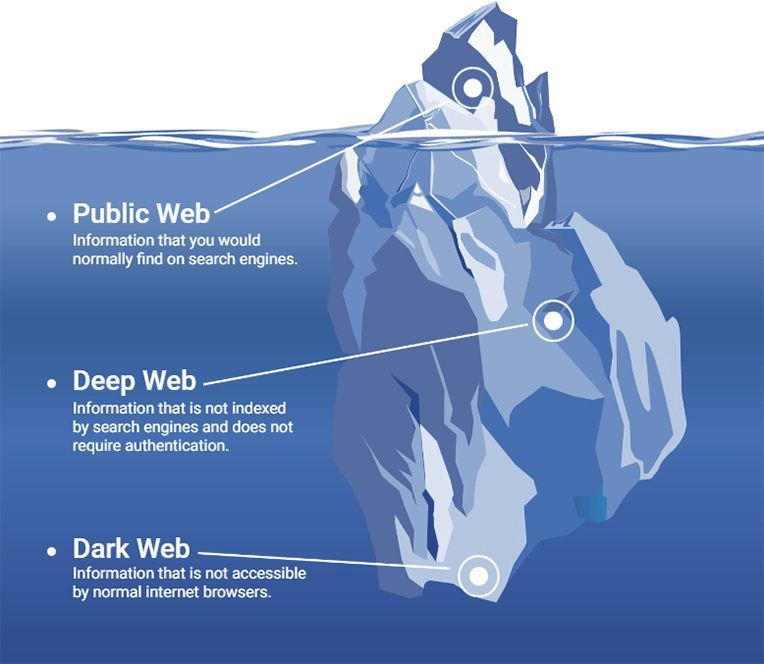
\includegraphics[width=\paperwidth,height=1.05\paperheight]{DarkNet}\hfill}}	
	}%
\begin{frame}
\end{frame}
}

\begin{frame}
	\frametitle{Darknet}
	
	Used interchangeably in this work:
	\vfill
	
	\begin{minipage}{.6\pagewidth}
	\begin{itemize}\setlength\itemsep{1em}
	\item \textbf{Dark Web}
	\item \textbf{Darknet}
	\item \textbf{Tor} network (Tor: an encrypted browser)
	\item \textbf{Onion} network (.onion top-level domain)
	\end{itemize}
	\end{minipage}
	\begin{minipage}{.3\pagewidth}
	
\includegraphics[width=.3\pagewidth]{Tor.png}
	\end{minipage}
	\vfill
	
	Hosts: \textbf{onion services} (hidden services).
\end{frame}

\begin{frame}
	\frametitle{Darknet Markets}
	
	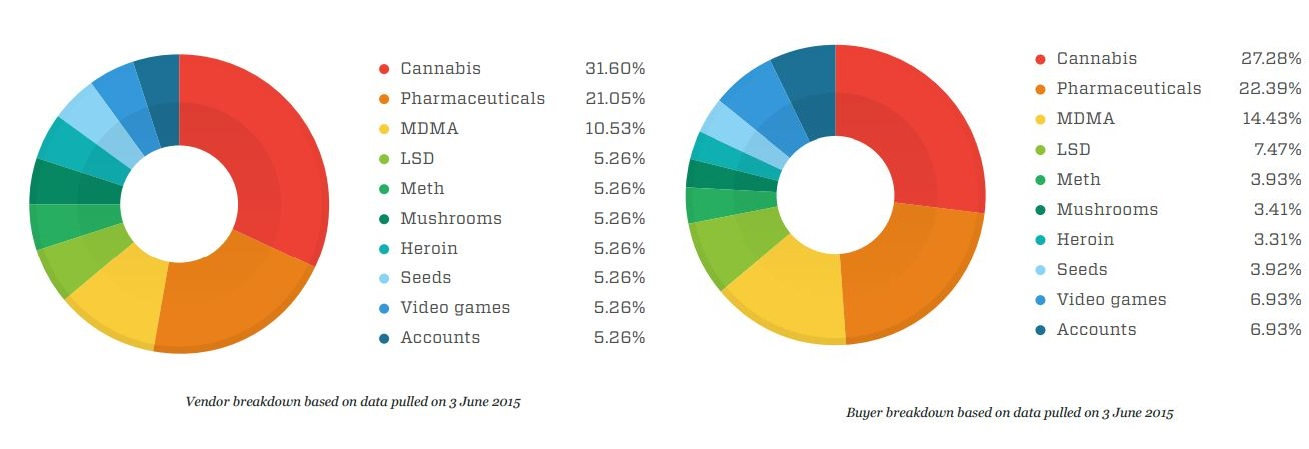
\includegraphics[trim={0 2cm 16cm 1cm},clip,width=\pagewidth]{DeepWeb-Black-markets-vendors-buyers.jpg}\footnote{Paganini (2015). "The Deep Web and Its Darknets".}
\end{frame}

\begin{frame}
	\frametitle{Language of the Darknet}
	
	\begin{center}
	How well do \textbf{NLP tools} work on Darknet text?
	
\includegraphics[width=.4\textwidth]{spacy.png}
	\vfill
	\pause
	
	Can we automatically \textbf{identify} illegal activity?
	
\includegraphics[width=.4\textwidth]{illegal.jpg}
	
	Disclaimer:
	variations among legal systems, societies and groups.
	\end{center}
\end{frame}

\section{Data}

\begin{frame}
	\frametitle{DUTA-10K}
	
	Dataset of 10367 Onion Services text pages \cite{AlNabki19}.

	\begin{itemize}\setlength\itemsep{1em}
		\item Classified by monitoring needs of Spanish \textbf{law enforcement agencies}.
		\item 20\% categorized as \textbf{illegal} and 48\% as \textbf{legal} (32\% unavailable).
		\item Of the illegal websites, 23\% concern illegal \textbf{drugs}.
	\end{itemize}
	\vfill
	\pause

	Distribution of categories:
	
	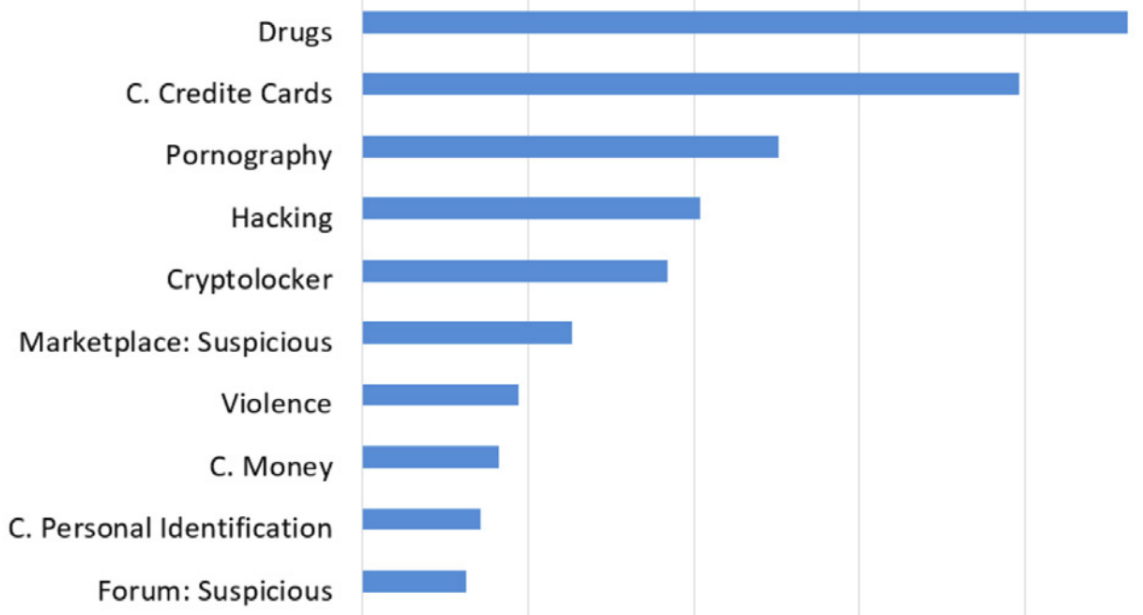
\includegraphics[width=.49\textwidth]{suspicious.png}\hfill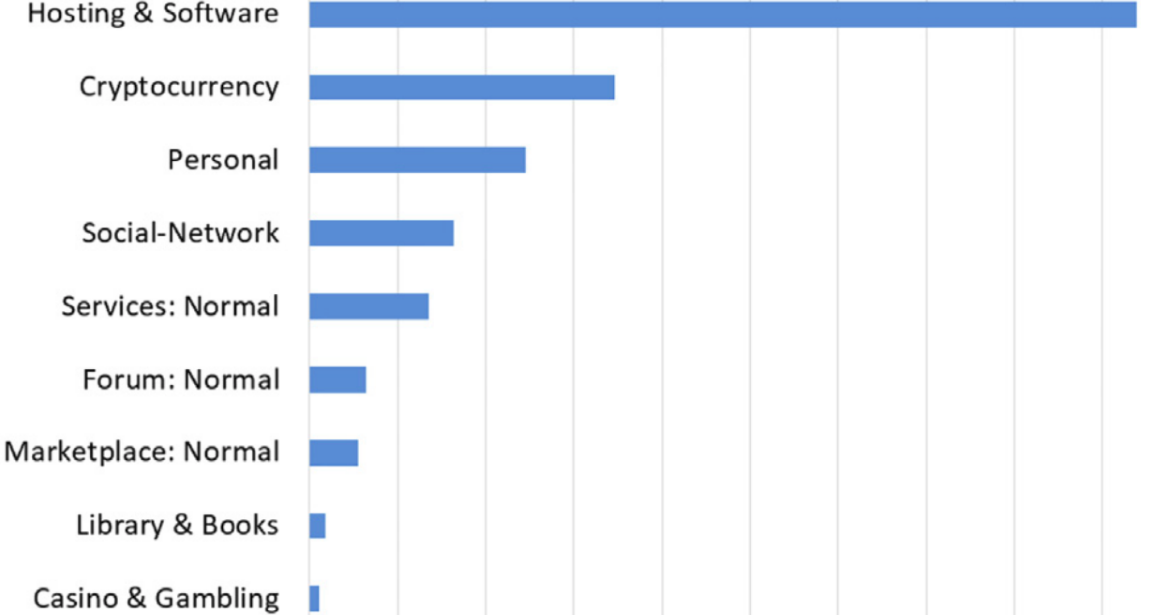
\includegraphics[width=.49\textwidth]{normal.png}
	
	\hspace{2cm} Illegal \hspace{5cm} Legal
\end{frame}

\setbeamercolor{background canvas}{bg=black}
\begin{frame}[fragile]
	\small
	\begin{center}\color{OwlGreen}
		\begin{verbatim}
			Finest organic cannabis grown by proffessional growers in the
			netherlands.
			We double seal all packages for odor less delivery.
			Shipping within 24 hours!
			              Product                    Price          Quantity
			1g Original Haze                    15 EUR = 0.025 ฿ 1_ X Buy now
			5g Original Haze                    65 EUR = 0.108 ฿ 1_ X Buy now
			1g Bubblegum                        10 EUR = 0.017 ฿ 1_ X Buy now
			5g Bubblegum                        45 EUR = 0.075 ฿ 1_ X Buy now
			1g Jack Herer                       14 EUR = 0.023 ฿ 1_ X Buy now
			5g Jack Herer                       60 EUR = 0.099 ฿ 1_ X Buy now
			1g Chronic                          9 EUR = 0.015 ฿  1_ X Buy now
			5g Chronic                          40 EUR = 0.066 ฿ 1_ X Buy now
			1g Banana Kush                      11 EUR = 0.018 ฿ 1_ X Buy now
		\end{verbatim}
	\end{center}
\end{frame}

\setbeamercolor{background canvas}{bg=white}
\begin{frame}[fragile]
	\frametitle{Control Data: eBay}
	Product descriptions acquired by searching for drug-related terms.
	\vfill
	
	Do not sell actual drugs, but rather drug-related products.
	\vfill
	
	\begin{center}
	
\includegraphics[width=.5\textwidth]{ebay.png}
	\end{center}
	\vfill
	
	\small
	\begin{center}\color{green}
		\begin{verbatim}
			3 Layers  Chip Style Herb Herbal Tobacco Grinder Weed Grinders
			Description:
			Quantity: 1
			Type : Tobacco Crusher
			Feature: Stocked,Eco-Friendly
			Material: plastic
			Size: 42*26mm
			Package include:
			1PC  Tobacco Crusher
		\end{verbatim}
	\end{center}
\end{frame}

\begin{frame}
	\frametitle{Data}
	
	\begin{center}
	\def\arraystretch{2}
	\begin{tabular}{c|ccc}
	& Public Web && Dark Web \\ 
	\hline
	\multirow{2}{*}{Legal} & \textbf{\color{yellow} eBay} && \textbf{\color{green} Legal Onion} \\
	& (188 pages, 35,799 words) && (35 pages, 61,655 words) \\\\
	\multirow{2}{*}{Illegal} &&& \textbf{\color{red} Illegal Onion} \\
	&&& (255 pages, 1,438,351 words)
	\end{tabular}
	\end{center}
\end{frame}

\begin{frame}[fragile]
	\frametitle{Cleaning}
	\begin{itemize}\setlength\itemsep{1em}
	\item Remove non-linguistic content: buttons, encryption keys, URLs...
	\item Split to paragraphs, join to single lines, remove duplicates.
	\item Sampled 571 paragraphs from each, for comparable size.
	
\includegraphics[width=.2\textwidth]{pipette.png}

	\end{itemize}
\end{frame}

\section{Domain Differences}

\begin{frame}
	\frametitle{Vocabulary}
	
	\begin{flushright}
	\tt\small\rowcolors{1}{lightgray!60}{lightgray!30}
	\setlength{\tabcolsep}{2pt}
	\begin{tabular}{||lr|}
	\hline
	to & 0.0486 \\
	the & 0.4242 \\
	of & 0.0162 \\
	is & 0.0118 \\
	and & 0.0102 \\
	\ldots & \\
	EUR & 0.0094 \\
	cocaine & 0.0041 \\
	Free & 0.0041 \\
	drug & 0.0035 \\
	1 & 0.0025 \\
	\ldots & \\
	\hline
	\end{tabular}
	\end{flushright}
	\vspace{-55mm}
	
	Distance between word distributions\pause, measured by:
	\begin{minipage}{.43\textwidth}
		\begin{itemize}
			\item Jensen-Shannon divergence
		\end{itemize}
	\end{minipage}
	\begin{minipage}{.3\textwidth}
		\begin{itemize}
			\item L1 distance
		\end{itemize}
	\end{minipage}
	\vfill
	
	Small ``self-distances'', found by splitting each in half{\pause}, \\ 
	but the different domains are about equidistant.
	
	\begin{center}
	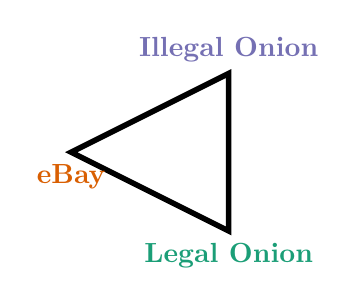
\begin{tikzpicture}
	\draw[line width=2] (0,1) node[anchor=north]{\textbf{\color{yellow} eBay}}
	  -- (2,0) node[anchor=north]{\textbf{\color{green} Legal Onion}}
	  -- (2,2) node[anchor=south]{\textbf{\color{red} Illegal Onion}}
	  -- cycle;
	\end{tikzpicture}
	\end{center}
	\pause
	
	Legal and illegal Onion should be considered different domains.
\end{frame}

\begin{frame}
	\frametitle{Characteristics of Darknet Data}
	
	Diverse: sub-domains are distinguishable.
	\vfill
	
	Unique: distinguishable from other domains.
	
	\begin{figure}
		\centering
		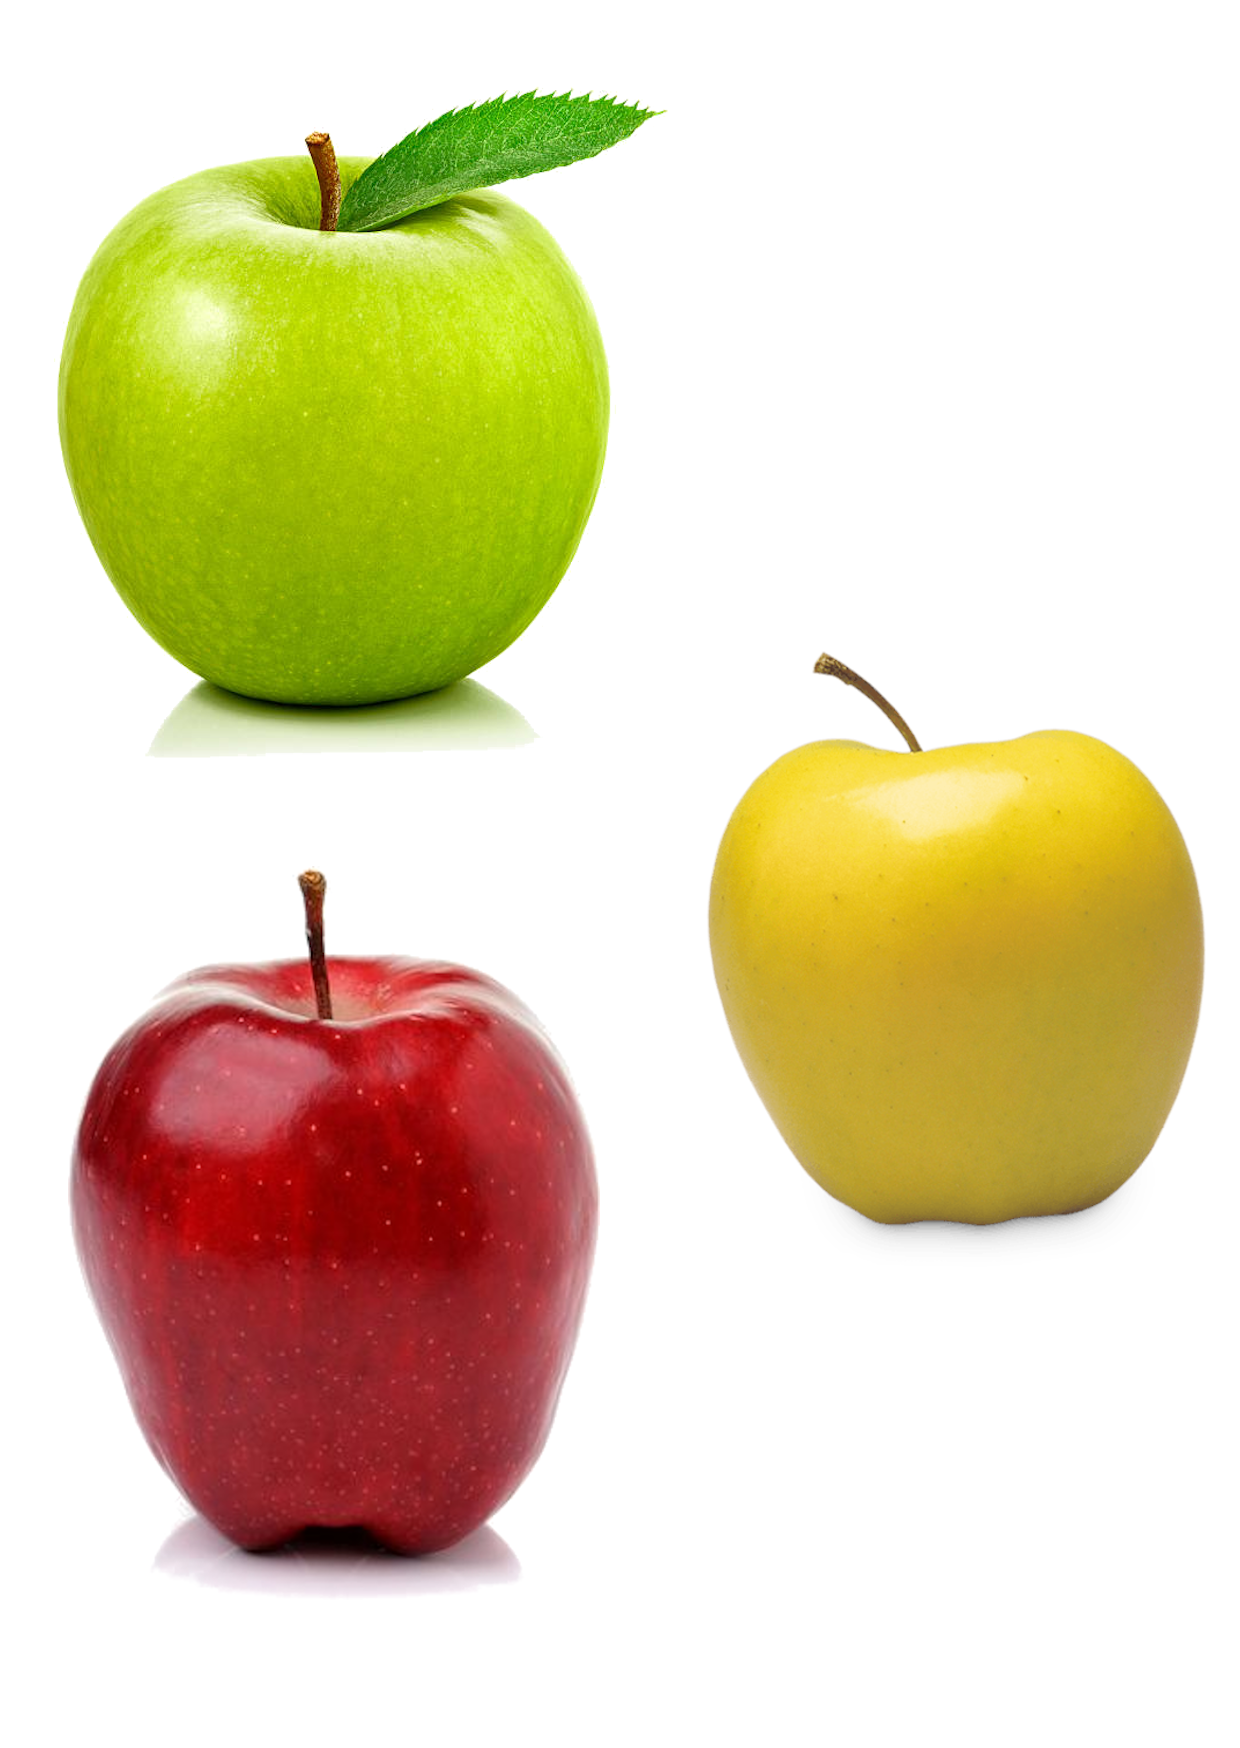
\includegraphics[width=0.3\textwidth]{3different.png}
	\end{figure}
\end{frame}

\begin{frame}
	\frametitle{Named Entities and Wikification}
	
	NE extraction [spaCy] + Wikification \cite{bunescu2006using}.
	\vfill
	
	\begin{center}
	\begin{tabular}{l|c}
	 & \% (of detected NEs) Wikifiable\\
	 \hline
	\textbf{\color{yellow} eBay} & $38.6 \pm2.00$\\
	\textbf{\color{red} Illegal Onion} & $32.5 \pm1.35$\\
	\textbf{\color{green} Legal Onion} & $50.8 \pm2.31$
	\end{tabular}
	\end{center}
	\vfill

	By manual inspection, NE precision and recall are low for \textbf{\color{red} Illegal Onion}.
	
	For example: slang words for drugs (e.g., ``\textbf{\color{red} kush}'') falsely picked up as NEs.	
	\vfill
	
	$\Rightarrow$ Standard NLP is not suited for this domain.
\end{frame}

\section{Classification}

\begin{frame}
	\frametitle{Classes}
	We identified three domains. Two binary classification settings:
	\begin{center}
	\{ \textbf{\color{yellow} eBay}, \textbf{\color{green} Legal Onion} \}
	\vfill
	
	\{ \textbf{\color{green} Legal Onion}, \textbf{\color{red} Illegal Onion} \}
	\end{center}
	\vfill
	\pause
	
	What are the linguistic features distinguishing them?
	\vfill
	
	\begin{center}
	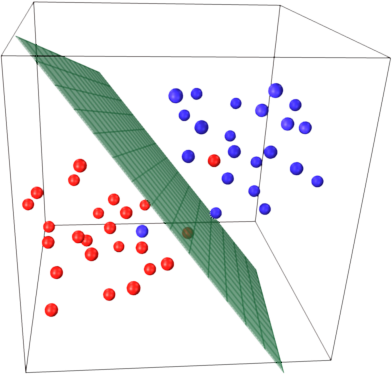
\includegraphics[width=.3\textwidth]{svm.png}
	\end{center}
\end{frame}

\begin{frame}
	\frametitle{Classifiers}
	
	\begin{minipage}{.7\textwidth}
	\begin{itemize}\setlength\itemsep{1em}
		\item NB: Naive Bayes (bag of words)
		\item SVM: Support Vector Machine
		\item BoE: sum/average GloVe + MLP
		\item seq2vec: BiLSTM + MLP
		\item attention: ELMo + BCN (self-attention)
	\end{itemize}
	\end{minipage}
	\begin{minipage}{.29\textwidth}
	\centering
	\hspace{-2cm}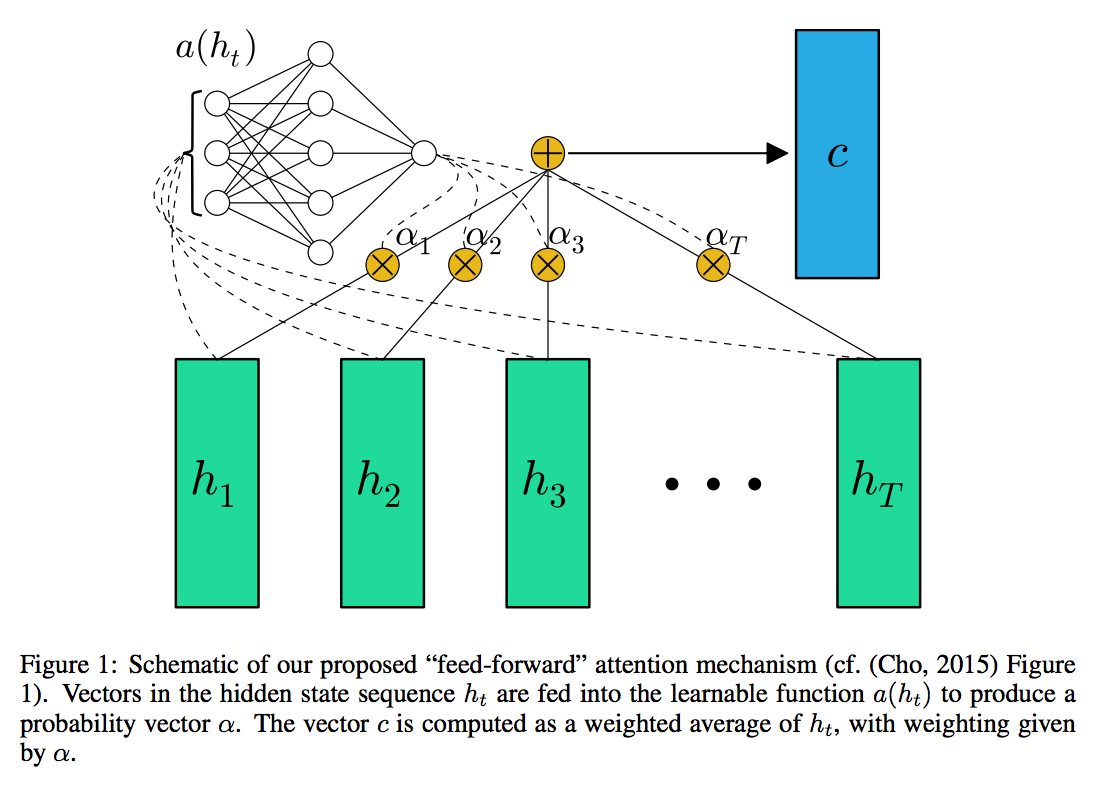
\includegraphics[trim={3cm 3cm 3cm 0},clip,width=1.5\textwidth]{FeedForwardAttention.png}
	
	
\includegraphics[width=.7\textwidth]{elmo.jpg}
	\end{minipage}
\end{frame}

\begin{frame}
	\frametitle{Manipulations}
	
	What are the linguistic cues used for classification?
	\pause
	Conditions:
	\vfill
	
	\begin{itemize}\setlength\itemsep{1em}
	    \item Full original text
	\end{itemize}
	\vspace{1em}
	
	\begin{minipage}{.35\textwidth}
	\begin{itemize}\setlength\itemsep{1em}
		\item Drop \textbf{content} words
		\item Drop \textbf{function} words
	\end{itemize}
	\end{minipage}
	\begin{minipage}{.59\textwidth}
	\begin{itemize}\setlength\itemsep{1em}
		\item \only<3->{\ul}{Replace \textbf{content} words with their POS}
		\item Replace \textbf{function} words with their POS
	\end{itemize}
	\end{minipage}
	\vfill
	
    \[\{\textsc{adj, adv, noun, propn, verb, x, num}\}\]
	\vfill
	\pause
	
	{\color{green}
	\setlength{\tabcolsep}{2.3pt}
	\begin{tabular}{ccccccccccc}
	Generic&Viagra&(&Oral&Jelly&)&is&used&for&Erectile&Dysfunction\\
	\small\textsc{propn} & \small\textsc{propn} &(& \small\textsc{propn} & \small\textsc{propn} &)& \small\textsc{verb} & \small\textsc{verb} & for & \small\textsc{propn} & \small\textsc{propn}
	\end{tabular}}
	\vfill
	\pause
	
	{\color{red}
	\setlength{\tabcolsep}{9.5pt}
	\begin{tabular}{ccccccc}
	Welcome&to&SnowKings&Good&Quality&Cocaine&!\\
	\small\textsc{verb} & to & \small\textsc{propn} & \small\textsc{propn} & \small\textsc{propn} & \small\textsc{propn} & !
	\end{tabular}}
\end{frame}

\begin{frame}
	\frametitle{Results}
	
	\textbf{\color{yellow} eBay} vs. \textbf{\color{green} Legal Onion} drugs:
	
	\begin{center}
		\setlength{\tabcolsep}{8pt}\def\arraystretch{1.8}
		\begin{tabular}{l *{5}{R}}
		& \multicolumn{1}{c}{\bf \rotatebox{90}{full}}
		& \multicolumn{1}{c}{\bf \rotatebox{90}{drop}\rotatebox{90}{content}}
		& \multicolumn{1}{c}{\bf \rotatebox{90}{drop}\rotatebox{90}{function}}
		& \multicolumn{1}{c}{\bf \rotatebox{90}{pos}\rotatebox{90}{content}}
		& \multicolumn{1}{c}{\bf \rotatebox{90}{pos}\rotatebox{90}{function}}\\
		\hline
		NB & 91.4 & 57.8 & 90.5 & 56.9 & 92.2\\
		SVM & 63.8 & 64.7 & 63.8 & 68.1 & 63.8\\
		BoE$_\mathrm{sum}$ & 66.4 & 56.0 & 63.8 & 50.9 & 76.7\\
		BoE$_\mathrm{average}$ & 75.0 & 55.2 & 59.5 & 50.0 & 75.0\\
		seq2vec & 73.3 & 53.8 & 65.5 & 65.5 & 75.0\\
		attention & 82.8 & 57.5 & 85.3 & 62.1 & 82.8
		\end{tabular}
	\end{center}
\end{frame}

\begin{frame}
	\frametitle{Results}
	
	\textbf{\color{green} Legal Onion} vs. \textbf{\color{red} Illegal Onion} drugs:
	
	\begin{center}
		\setlength{\tabcolsep}{8pt}\def\arraystretch{1.8}
		\begin{tabular}{l *{5}{R}}
		& \multicolumn{1}{c}{\bf \rotatebox{90}{full}}
		& \multicolumn{1}{c}{\bf \rotatebox{90}{drop}\rotatebox{90}{content}}
		& \multicolumn{1}{c}{\bf \rotatebox{90}{drop}\rotatebox{90}{function}}
		& \multicolumn{1}{c}{\bf \rotatebox{90}{pos}\rotatebox{90}{content}}
		& \multicolumn{1}{c}{\bf \rotatebox{90}{pos}\rotatebox{90}{function}}\\
		\hline
		NB & 77.6 & 53.4 & 87.9 & 51.7 & 77.6\\
		SVM & 63.8 & 66.4 & 63.8 & 70.7 & 63.8\\
		BoE$_\mathrm{sum}$ & 52.6 & 61.2 & 74.1 & 50.9 & 51.7\\
		BoE$_\mathrm{average}$ & 57.8 & 57.8 & 52.6 & 55.2 & 50.9\\
		seq2vec & 56.9 & 55.0 & 54.3 & 59.5 & 49.1\\
		attention & 64.7 & 51.4 & 62.9 & 55.2 & 69.0
		\end{tabular}
	\end{center}
\end{frame}

\section{Cross-Domain Classification}

\begin{frame}
	\frametitle{Darknet Forums}
	
	Can we generalize beyond drugs?
	\vfill
	\pause
	
	DUTA-10K also contain
	{\color{green}Legal Forums} and {\color{red}Illegal Forums}.
	
	Multi-topic and user-generated.
	\vfill
	
	\begin{center}
	
\includegraphics[width=.5\textwidth]{forum.jpg}
	\end{center}
\end{frame}

\begin{frame}
	\frametitle{Results}
	
	\textbf{\color{green} Legal Onion} vs. \textbf{\color{red} Illegal Onion} forums:
	
	\begin{center}
		\setlength{\tabcolsep}{8pt}\def\arraystretch{1.8}
		\begin{tabular}{l *{5}{R}}
		& \multicolumn{1}{c}{\bf \rotatebox{90}{full}}
		& \multicolumn{1}{c}{\bf \rotatebox{90}{drop}\rotatebox{90}{content}}
		& \multicolumn{1}{c}{\bf \rotatebox{90}{drop}\rotatebox{90}{function}}
		& \multicolumn{1}{c}{\bf \rotatebox{90}{pos}\rotatebox{90}{content}}
		& \multicolumn{1}{c}{\bf \rotatebox{90}{pos}\rotatebox{90}{function}}\\
		\hline
		NB & 74.1 & 50.9 & 78.4 & 50.9 & 72.4\\
		SVM & 85.3 & 75.9 & 56.0 & 81.9 & 81.0\\
		BoE$_\mathrm{sum}$ & 25.9 & 32.8 & 21.6 & 36.2 & 35.3\\
		BoE$_\mathrm{average}$ & 40.5 & 42.2 & 31.9 & 48.3 & 53.4\\
		seq2vec & 50.0 & 48.9 & 50.9 & 28.4 & 51.7\\
		attention & 31.0 & 37.2 & 33.6 & 27.6 & 30.2
		\end{tabular}
	\end{center}
\end{frame}

\begin{frame}
	\frametitle{Results}
	
	Trained on \textbf{drugs},
	evaluated on \textbf{forums} (\textbf{\color{green} Legal Onion} vs. \textbf{\color{red} Illegal Onion}):
	
	\begin{center}
		\setlength{\tabcolsep}{8pt}\def\arraystretch{1.8}
		\begin{tabular}{l *{5}{R}}
		& \multicolumn{1}{c}{\bf \rotatebox{90}{full}}
		& \multicolumn{1}{c}{\bf \rotatebox{90}{drop}\rotatebox{90}{content}}
		& \multicolumn{1}{c}{\bf \rotatebox{90}{drop}\rotatebox{90}{function}}
		& \multicolumn{1}{c}{\bf \rotatebox{90}{pos}\rotatebox{90}{content}}
		& \multicolumn{1}{c}{\bf \rotatebox{90}{pos}\rotatebox{90}{function}}\\
		\hline
		NB & 78.4 & 63.8 & 89.7 & 63.8 & 79.3\\
		SVM & 62.1 & 69.0 & 54.3 & 69.8 & 62.1\\
		BoE$_\mathrm{sum}$ & 45.7 & 50.9 & 49.1 & 50.9 & 50.0\\
		BoE$_\mathrm{average}$ & 49.1 & 51.7 & 51.7 & 52.6 & 58.6\\
		seq2vec & 51.7 & 61.1 & 51.7 & 54.3 & 57.8\\
		attention & 65.5 & 59.2 & 65.5 & 50.9 & 66.4
		\end{tabular}
	\end{center}
\end{frame}

\section*{}

\begin{frame}
	\frametitle{Conclusion}
	Differences between legal and illegal Darknet sites include:
	
	Vocabulary,
	shallow syntax (POS)
	and named entities.
	\vfill
	\pause
	
	Identified by:
	\begin{itemize}\setlength\itemsep{1em}
	\item Word statistics: diverse and unique
	\item Wikification: works less well on illegal
	\item Predictive: simple classifiers work best
	\end{itemize}
	\vfill
	\pause
	
	Social implications, as well as implications for law enforcement.
	\vfill
	\pause
	
	\begin{minipage}{.7\textwidth}
	\color{blue}\url{https://github.com/huji-nlp/cyber}
	\end{minipage}
	\pause
	\begin{minipage}{.28\textwidth}
	\centering\vspace{-2cm}
	
\includegraphics[width=.8\textwidth]{onion.jpg}
	
	Thanks!
	\end{minipage}
\end{frame}

\begin{frame}[allowframebreaks]
\frametitle{References}
\bibliographystyle{apalike}
\tiny\bibliography{acl2019}
\end{frame}

\end{document}
